\documentclass[9pt,twocolumn,twoside]{rilabRxiv}
% Use the documentclass option 'lineno' to view line numbers
\setlength{\marginparwidth}{2cm}
\usepackage[textsize=tiny,colorinlistoftodos]{todonotes} % comments in margins
\definecolor{cornflowerblue}{rgb}{0.39, 0.58, 0.93}
\usepackage{blindtext}


%%%%%%%Add comments in color
\newcommand{\ms}[1]{{\small \textcolor{green}{#1}}}
\newcommand{\jri}[1]{{\small \textcolor{red}{#1}}}
\newcommand{\citex}[1]{{\small \textcolor{red}{CITE(#1)}}}
\newcommand{\X}{{\textcolor{red}{X}}}

\newcolumntype{b}{X}
\newcolumntype{s}{>{\hsize=.5\hsize}X}

% Set supplement numbers to S and start counting newly
\newcommand{\beginsupplement}{%
        \setcounter{table}{0}
        \renewcommand{\thetable}{S\arabic{table}}%
        \setcounter{figure}{0}
        \renewcommand{\thefigure}{S\arabic{figure}}%
     }


\usepackage{hyperref}

\title{Latex template for bioRxiv articles}

\author[$\ast$,1]{First Author}
\author[$\dagger$]{Second Author}
\author[$\ast$,$\ddagger$,1]{Third Author}


\affil[$\ast$]{Dept. of Plant Sciences and Center for Population Biology, University of California, Davis, CA, USA}
\affil[$\dagger$]{Some other Department, Some other place, CA, USA}
\affil[$\ddagger$]{Genome Center, University of California, Davis, CA, USA}


\keywords{Keyword one, keyword 2}

\runningtitle{Running title} % For use in the footer

%% For the footnote.
%% Give the last name of the first author if only one author;
% \runningauthor{FirstAuthorLastname}
%% last names of both authors if there are two authors;
% \runningauthor{FirstAuthorLastname and SecondAuthorLastname}
%% last name of the first author followed by et al, if more than two authors.
\runningauthor{One \textit{et al.}}


%%% Abstract %%%%%%%%%%%%%%%%%%
\begin{abstract}
Write your abstract in here 
\blindtext
\end{abstract}
%%%%%%%%%%%%%%%%%%%%%%%%%%


\setboolean{displaycopyright}{true}

\begin{document}

\maketitle
\thispagestyle{firststyle}
%\firstpagefootnote
\correspondingauthoraffiliation{
Dept. of Plant Sciences, University of California, Davis, CA, USA
E-mail: corresponding@ucdavis.edu}
\vspace{-11pt}%

\section{Introduction}
\subsection{First part}
\lettrine[lines=2]{\color{color2}A}{} good introduction is very important.
This is how you can \citet{hufford2012comparative} in line or as reference in the end \citep{bourne2017ten}.
\subsection{Second part}
\blindtext
\section{Materials and Methods}
\label{sec:materials:methods}

This is an example table 
%\textbf{General}
\begin{table}[htbp]
\centering
\caption{\bf Parameters and variables}
\begin{tableminipage}{0.5\textwidth}
\begin{tabularx}{\textwidth}{sb}
\hline
 Variable & Description \\
\hline
$N_{anc}$ & Population size at equilibrium \\
$N_{final}$ & Population size after 0.1 * $N_{anc}$ generations \\
$N_{bottlenck}$ & Population size during bottleneck \\
$\psi$ & Genetic background proportion \\
$\sigma_m$ & Standard deviation of effect sizes of new mutations \\
$V_S$ & Strength of stabilizing selection \\
$V_{G0}$ & Genetic variance at equilibrium\\
\hline
\end{tabularx}
  \label{tab:shape-functions}
\end{tableminipage}
\end{table}

\subsection{Experiment 1}
\blindtext

\subsubsection{Experiment 2}
This is an example equation

\begin{equation}
\label{eqn:fitness}
w =exp [-\frac{(z-z_{opt})^2}{2V_S}]
\end{equation}

\blindtext
%%%%%%%%%%%%%%%%%%%%%%%%%%%%%%%%%%%%%%%%%%%%%%%%%%%%%%
\section{Results}
%%%%%%%%%%%%%%%%%%%%%%%%%%%%%%%%%%%%%%%%%%%%%%%%%%%%%%

Here is a single column figure (Figure \ref{fig:figure1})

\begin{figure}[ht]

\includegraphics[width=0.6\linewidth]{figures/jri_bee.jpg}
\caption{\textbf{Important figure} Describe the figure }
\label{fig:figure1}
\end{figure}

\blindtext

\blindtext
\blindtext
\blindtext
\blindtext
%%%%%%%%%%%%%%%%%%%%%%%%%%%%%%%%%%%%%%%%%%%%%%%%%%%%%%
\section{Discussion}
%%%%%%%%%%%%%%%%%%%%%%%%%%%%%%%%%%%%%%%%%%%%%%%%%%%%%%
\subsection{Some more test}
\blindtext
\blindtext


\subsection{another figure}
This is a full size figure (Figure \ref{fig:S1}) just add stars to the figure


\section{Acknowledgments}
We acknowledge the support of our coffee maker that made this work possible

\bibliography{example-bibliography}

%\pagebreak
\onecolumn
\section*{Supplement}


     
\beginsupplement


\blindtext
\begin{figure*}[h!]
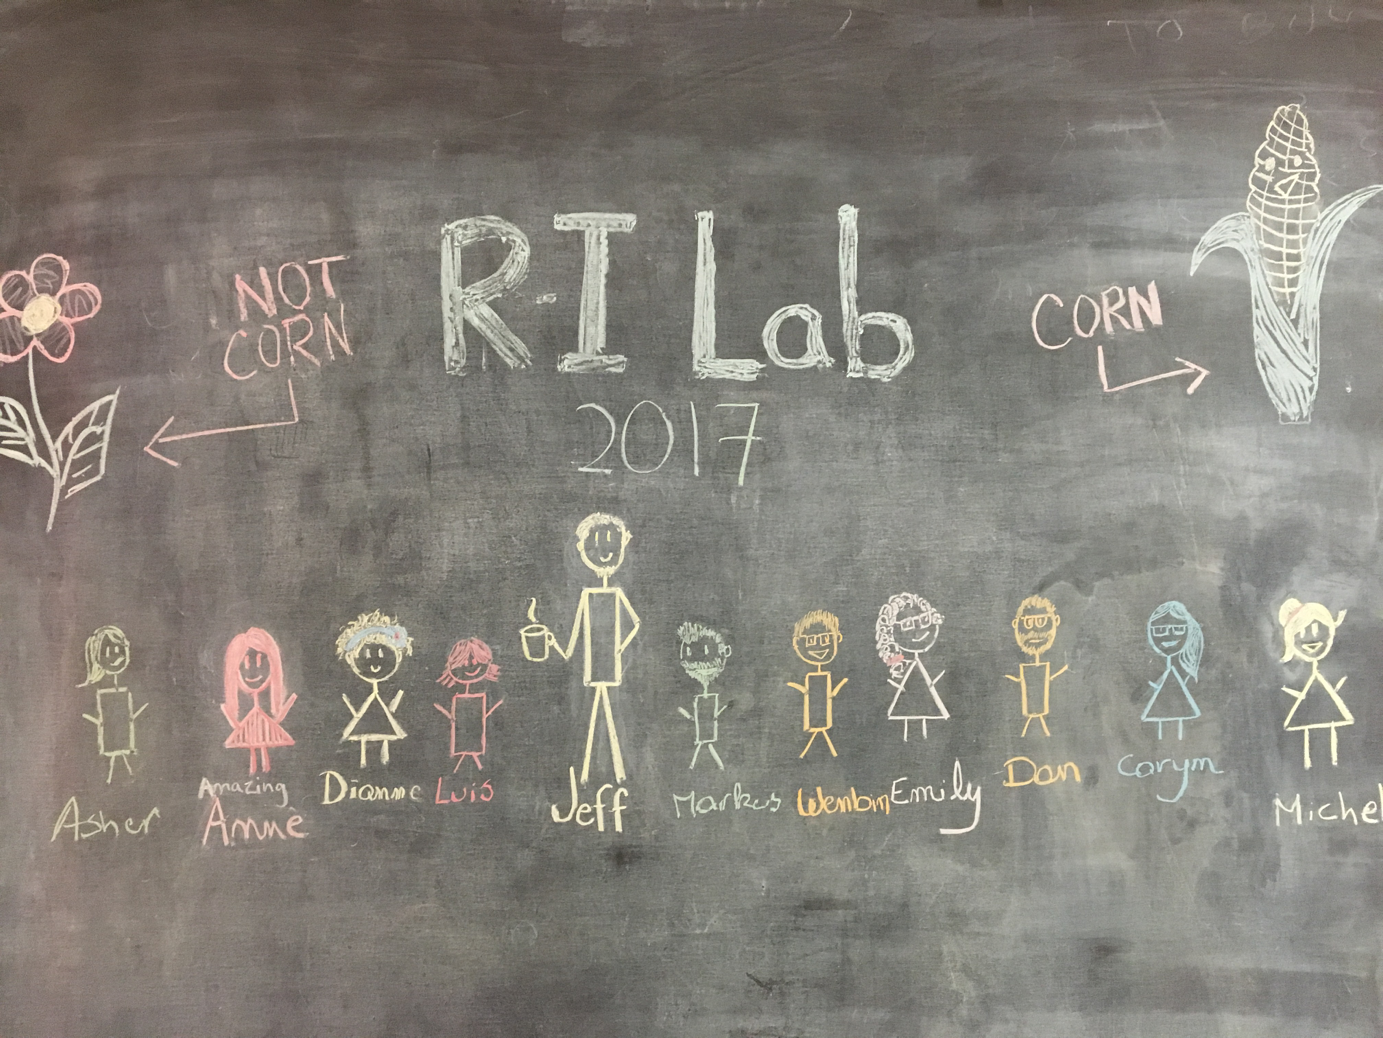
\includegraphics[width=.9\linewidth]{figures/lab_group.png}
\caption{\textbf{Supplemental figure} Test test test}
\label{fig:S1}
\end{figure*}
\pagebreak




\begin{table*}[htbp]
\centering

\caption{\bf Shrink a large table to fit the page}
%\begin{adjustbox}{totalheight=\textheight-2\baselineskip}
\begin{tableminipage}{\textwidth}
\begin{small}
\begin{tabularx}{\textwidth}{sb}
\hline
Parameter & Description \\
\hline
\textbf{Adaptation} & \textbf{Trait related parameters} \\
\hline
Time to optimum & Generations until new optimum is reached \\
Adaptation rate (haldane) & Adaptation rate until new optimum is reached. Calculated as $rate(h) = \frac{\frac{ln(x_2)}{sd_{x_{12}}}-\frac{ln(x_1)}{sd_{x_{12}}}}{t_2-t_1}$ \\
Final genetic variance & Genetic variance in the final generation \\
\textbf{Fixations} & \textbf{Mutations that fix after the optimum shift} \\
\hline
From new mutations (\#) & Sum of fixed mutations in the final population that were already segregating before  the optimum shift \\
From standing variation (\#) & Sum of fixed mutations in the final population that arose after the optimum shift \\
Max. effect size & Maximal effect size of all fixations \\
Mean effect size & Mean effect size of all fixations \\
Mean effect size of negative fixations & Mean effect size of negative mutations \\
Mean effect size of positive fixations & Mean effect size of positive mutations \\
Mean emergence time & Mean generation when a mutation arose that fixed in the last 0.1 N generations \\
Mean fixation time & Mean generation in which a mutation fixed \\
Min. effect size & Minimal effect size of all fixations \\
Negative (\#) & Sum of fixed mutations with negative effects in the final population \\
New/standing fixations & Ratio of mutations from new mutations vs. standing mutations  \\
Proportion negative & Proportion of negative fixations from all mutations \\
Positive (\#) & Sum of fixed mutations with positive effects in the final population \\
SD of effect sizes & Standard deviation of effect sizes of all fixations \\
SD of negative effect sizes & Standard deviation of effect sizes of negative fixations \\
SD of positive effect sizes & Standard deviation of effect sizes of positive fixations \\
Total (\#) & Sum of fixed mutations in the final population \\
\textbf{Sweeps} & \textbf{Mutations that fix faster than 99\% of neutral fixations} \\
\hline
Hard sweeps (\#) & Sum of selective sweeps from new mutations \\
Proportion of hard sweeps & Porportion of hard selective sweeps of all selective sweeps \\
Proportion of sweeps from standing & Proportion of selective sweeps from stainding variation of all selection sweeps \\
Sweeps (\#) & Sum of selective sweeps \\
Sweeps from standing variation (\#) & Sum of selective sweeps from mutations that were already segregating before  the optimum shift \\
Sweeps/fixations & Ratio of sweeps vs. fixations \\
\textbf{Segregating sites} & \textbf{Mutations that segregate in the final generation} \\
\hline
Max. effect size & Maximal effect size of segregating sites \\
Mean effect size & Mean effect size of segregating sites \\
Mean effect size of negative sites & Mean effect size of segregating sites with negative effects \\
Mean effect size of positive sites & Mean effect size of segregating sites with positive effects \\
Mean frequency of all sites & Mean allele frequency of segregating sites \\
Mean frequency of negative sites & Mean allele frequency of segregating sites with negative effects \\
Mean frequency of positive sites & Mean allele frequency of segregating sites with positive effects \\
Min. effect size & Minimal effect size of segregating sites \\
Negative (\#) & Sum of segregating sites with negative effect \\
Positive (\#) & Sum of segregating sites with positive effect \\
Proportion of negative sites & Proportion of segregating sites with negative effect of all segregating sites \\
Standard deviation of effect sizes & Standard deviation of effect sizes of all segregating sites \\
Total (\#) & Sum segregating sites in the final generation \\
\hline

\end{tabularx}
  \label{tab:parameter_list}
  \end{small}
\end{tableminipage}

%\end{adjustbox}
\end{table*}


\end{document}
